\documentclass[letter,10pt]{article}

\usepackage[latin1]{inputenc}
\usepackage[english]{babel}
\usepackage[T1]{fontenc}
\usepackage[dvips]{graphicx}
\usepackage[left=0.6in,right=0.6in,top=0.6in,bottom=0.6in]{geometry}
\usepackage{graphicx}
\usepackage{url}
\usepackage{wrapfig}
\usepackage{mhchem}

\title{Amateur Copper Smelting Experiments}
\author{Ryan R. Curtin, Joshua J. Cowan}
\date{\today}

\begin{document}
\maketitle

\begin{abstract}

\end{abstract}

\section{Introduction}

% The introduction.

% What is copper smelting?
% Why would someone want to do it?
% What useful products can be produced through copper smelting?

Copper is a particularly useful metal, widely used in all manner of applications
ranging from wire (due to its conductive characteristics) to roofing to use in
alloys, such as bronze, cupronickel, aluminum bronze, red brass, and many
others.  The use of copper dates back to antiquity, and the extraction of copper
from surface minerals by smelting dates back to at least 5000 BC.

% The above section needs some work...

% What techniques will be used to smelt this copper?


\section{Background}

% The background should contain a summarized history of the smelting and
% harvesting of copper dating from antiquity until now.  Environmental concerns
% should be minorly addressed and Ducktown provides a good example of that.  The
% modern techniques of copper smelting should be at least mentioned.


\section{Obtainment Of Ore}

% First, we should discuss the important copper deposits on the planet.

% Then, we should focus more on a local copper deposit -- the Copper Basin in
% north Georgia and southeastern Tennessee.

% A quick history of the Burra Burra mine should have been given in the
% background; at this point, the museum should be mentioned, and its open mining
% area discussed.

\subsection{Important Copper Deposits}

Copper is not a particularly rare mineral; however, its deposits on the surface
are somewhat limited to certain regions.  Among these regions are \textbf{some
places!} and a region in the southeastern United States known as the `Copper
Basin', located near the intersection of Georgia, North Carolina, and Tennessee.

...

\subsection{The `Copper Basin'}

...

\subsection{Collection of Ore}

Using the facilities at the Burra Burra Mine Museum as well as tools purchased
at the local hardware store (a sledgehammer, an axe, a shovel, and several large
buckets for storage and transport), a large quantity of chalcopyrite-containing
ore was collected.

Large rocks were repeatedly struck until shattering; this process was repeated
until the largest remaining chunks of ore were approximately 10 to 12 inches
across.  Then, each chunk was inspected.  A chunk was considered to contain a
high percentage of metallic material if visual inspection revealed high
quantities of small, reflective metallic crystals.  However, this strategy for
high-grade ore selection may not have been optimal.  Unfortunately, due to
museum-imposed timing constraints, a more accurate selection process was
infeasible.  A comparison of a high-grade ore to a low-grade ore (according to
our primitive heuristic) is given in Figure \ref{fig:ore-comparison}.  Any
chunks smaller than 10 to 12 inches across considered `high-grade' by our simple
methodology was collected, down to small gravel-sized pieces.

\begin{figure}[htb]
% subfigures will need to be used here.

\caption{Comparison of high-grade and low-grade ores (according to a primitive
heuristic).}
\label{fig:ore-comparison}

\end{figure}

In total, six ten-gallon buckets were filled with what was believed to be high
quality chalcopyrite ore.  In addition, because the Burra Burra Mine Museum also
made flux available (mostly quartz), two duffel bags were filled with flux, as
well as slag samples from earlier Burra Burra mine operations.  The weight of
the collected chalcopyrite ore was determined to be $440.4$ pounds, and the
weight of the collected flux was $138.0$ pounds.  This ore was transported back
to an undisclosed location north of the Georgia Tech campus.


\section{Ore Preparation}

% In this section we must discuss the preparation of the ore for roasting,
% including the Pulverator 9000.

Before the chalcopyrite ore can be roasted, it has to be prepared.  In our
setting, which is a far cry from the continual 240-ton roasts of the Burra Burra
mine (taking on the order of 70 to 80 days for a completed roast), a high
priority was a fast roasting process (3 to 4 hours).  Because the roasting
process simply involves burning the chalcopyrite ore to release the sulfur
dioxide, increasing the exposed surface area of the ore can greatly decrease the
roasting time.  Therefore, smaller chunks of chalcopyrite ore were necessary.

The simplest method for achieving this result would be the cathartic use of a
sledgehammer against the large ore chunks, fragmenting them into pieces of the
desired size.  However, this imparts high kinetic energy into each fragment, and
high-velocity losses can be difficult to recover.  With a limited amount of ore,
loss prevention was a high priority, and consequently, this simple fracturing
technique was considered unfitting.

To this end, the development of small-scale techniques for ore crushing (or
`spalling') with minimal losses was necessary.


\section{Roasting of Ore}

\subsection{Theory}

% Detail what is actually happening in this process.

The roasting process (also called calcining) is a preparation step before the
actual smelting and copper recovery process.  With chalcopyrite ore
(\ce{CuFeS2}), the effect of the process is to release one of the two sulfur
atoms as sulfur dioxide.  The stochiometry of the reaction is given in Equation
\ref{eq:roasting}.

\begin{equation}
\cee{2 CuFeS2 + 3 O2 -> 2 FeO + 2 CuS + 2 SO2}
\label{eq:roasting}
\end{equation}

This process is necessary to guarantee good smelting results.  During the
smelting process, free sulfur will first combine with elemental copper; however,
when the elemental copper is exhausted, remaining sulfur will next combine with
iron, thereby reducing the purity of the produced copper matte.  Therefore, if
too much sulfur is present in the smelted ore, it affects the results of the
whole smelting process adversely \cite{peters1887}.

The temperatures necessary for this reaction to occur are approximately
400$^\circ$C to 600$^\circ$C.  It is important that the temperature of the roast
not exceed the melting point of copper (above 1000$^\circ$C), or the risk of
premature and inconsistent smelting arises.

In some industrial settings, techniques such as froth flotation are first
performed on the raw ore to improve its purity; however, this technology is not
easily reproduced by amateurs (due in part to its dependence on industrial
chemicals) and for the purpose of this investigation is ignored.

\subsection{Heap Roasting}

The most primitive form of roasting is referred to as `heap roasting', and
involves simply placing crushed ore on top of fuel (generally wood, but charcoal
can also work) and lighting the fuel.  As the reduction process begins, which is
made obvious by the odiferous release of sulfur dioxide, the sulfur in the ore
will become the fuel for the reaction, and will burn with a small, easily
recognizable electric blue flame.

This simple technique has been practiced since antiquity, but the process
leading to its development is not known.  One theory suggests that the
spontaneous combustion of sulfide ores (due to the natural decay of the
sulfides) led a curious primitive metallurgist to inspect the results and
discover deposits of what appeared to be copper, or more likely copper matte,
caused by the temperatures of the spontaneous roasting reaching the melting
point of copper \cite{peters1887}.  Another theory suggests that early workers
found the ore easier to break into pieces after it was burned
% \cite{somewhere!}
.  A third theory proposes that inobservant metallurgists confused copper ore
for gold ore and, in burning it and finding unexpected results, discovered that
copper could be produced instead through that method
% \cite{where the hell did this come from?  I think I have the theory wrong}
.

Many things must be considered when roasting copper ore.  First, the location:
the roasting process releases sulfur dioxide (and other gases, which will be
described shortly), which is particularly destructive to the local environment
and is an irritant when inhaled.  A large enough cloud of sulfur dioxide could
even cause asphyxiation (due to oxygen starvation).  The next thing to consider
is the size of the roast heap.  In an industrial setting, heaps containing in
excess of hundreds of tons of ore were used; the sulfur-releasing roast would
continue for potentially months.  When applied to smaller scales, the roast time
seems to decrease accordingly.  The third thing to be considered is the size of
ore chunks to be roasted in this fashion; this parameter can vary wildly, from
small chunks of one-and-a-half inches in diameter to larger chunks of a foot or
more in diameter.  The size of the chunk, of course, affects the roasting time
greatly.

Because the calcining process occurs only on those parts of the rocks exposed to
heat, the interior of ore chunks tends to remain unroasted.  Therefore, the heap
should be stirred frequently.  Some chunks may break open during this process,
thereby exposing their interiors to the necessary heat for the reaction to
occur.  Similar to the culinary task of meat preparation, ores tend to roast
somewhat quickly on the exterior, forming a crust of FeO (the familiar
reddish-brown rust), and then the progress of the roasting inwards can be slow.

The criteria for evaluating the completeness of a roast are generally
particularly dependent on the specific ore as well as the patience levels of the
metallurgist.  Realistically a heap of sulfide ore could be continually kept at
the correct temperature for calcination without ill effects, until sulfur
dioxide emissions had dropped to virtually zero, allowing the conclusion to be
drawn that the process is entirely complete; however, the resources necessary
for this perfection (in both time and labor) are generally infeasible.

\subsection{Byproducts of Roasting}

Because most copper ore is not pure (i.e. only chalcopyrite or chalcocite),
several other byproducts are produced in the roasting process.  A report on the
minor minerals present at the Burra Burra mine in Ducktown sheds some light on
the impurities generally found with chalcopyrite deposits \cite{slater1980}.  A
few of these impurities are listed below (countless more have been omitted).

\begin{itemize}
   \item Magnetite (\ce{Fe3O4})
   \vspace{-1em}
   \item Sphalerite (\ce{ZnS})
   \vspace{-1em}
   \item Actinolite (\ce{Ca2(Fe, Mg)5(Si8O22)(OH)2})
   \vspace{-1em}
   \item Calcite (\ce{CaCO3})
   \vspace{-1em}
   \item Biotite (\ce{K(Mg, Fe)3(AlSi3O10)(OH)2})
   \vspace{-1em}
   \item Pyrite (\ce{FeS2})
   \vspace{-1em}
   \item Arsenopyrite (\ce{FeAsS})
   \vspace{-1em}
   \item Galena (\ce{PbS})
\end{itemize}

Of particular interest in that list are galena (\ce{PbS}) and arsenopyrite
(\ce{FeAsS}), which contain two elements known to be harmful to humans -- lead
and arsenic.  The list of symptoms for either lead or arsenic poisoning are
generally long and unhappy; long-term effects of lead and arsenic exposure are
never beneficial, and some even suppose that lead exposure led indirectly to the
decline of the Roman Empire \cite{angier2007}. % Yeah, really.

The roasting of arsenopyrite results in the reaction shown in Equation
\ref{eq:arsenopyrite}.  The only non-harmful substance produced by that reaction
is \ce{Fe2O3}, a form of rust.  Arsenopyrite is generally present in copper ores
(though in trace quantities), so any metallurgist should be aware that during
the roasting process arsenic trioxide is released.  Care should be taken to avoid
inhalation of the sulfur dioxide plume; this undoubtedly contains trace amounts
of arsenic trioxide, which is certainly not beneficial from a medicinal
perspective.

\begin{equation}
\label{eq:arsenopyrite}
\cee{2FeAsS2 + 5O2 -> Fe2O3 + 2SO2 + As2O3}
\end{equation}

The other trace mineral of interest is galena, a lead sulfide.  The reaction
produced by the roasting of galena is specified in Equation \ref{eq:galena}.
The only gas produced by this reaction is sulfur dioxide; so, no gaseous lead
compounds are released.  Nonetheless, PbO is now present in the roasted ore.

\begin{equation}
\label{eq:galena}
\cee{2PbS + 3O2 -> 2PbO + 2SO2}
\end{equation}

Only two byproducts of roasting have been examined in detail here.  The exact
and full list of byproducts is dependent on the exact ore sample.  Even so, more
gases than just sulfur dioxide (and trace amounts of arsenic trioxide) are being
released; with high probability, other harmful gases are also being released.

\subsection{Environmental Impact}

The release of sulfur dioxide is well-known to be entirely detrimental to the
environment.  The combination of sulfur dioxide and moisture produces sulfuric
acid---or acid rain---which then falls from the sky and corrodes its
destination, whether that is plant life, geologic structures, or manmade
artifacts (or even lifeforms).

% Quick discussion of what happened at Ducktown and a reference to other
% sources.

\subsection{Experimental Setup}

For the purposes of this series of experiments, the ore was split into batches
of 15 to 40 pounds and heap roasted inside of a brick structure with forced
airflow, fueled by charcoal.  Different configurations of forced airflow and
fueling mechanisms were tried; however, unfortunately, the quality of results
could not be assessed until the smelting stage -- by which point the batches of
roasted ore had been recombined.  Four heap roast configurations are shown in
Figure \ref{fig:heaproast}.

% Subfigures will be necessary.
\begin{figure}[htb]
\centering
\subfigure[First configuration.  Entirely enclosed.  Airflow provided through
holes in brick walls.]{
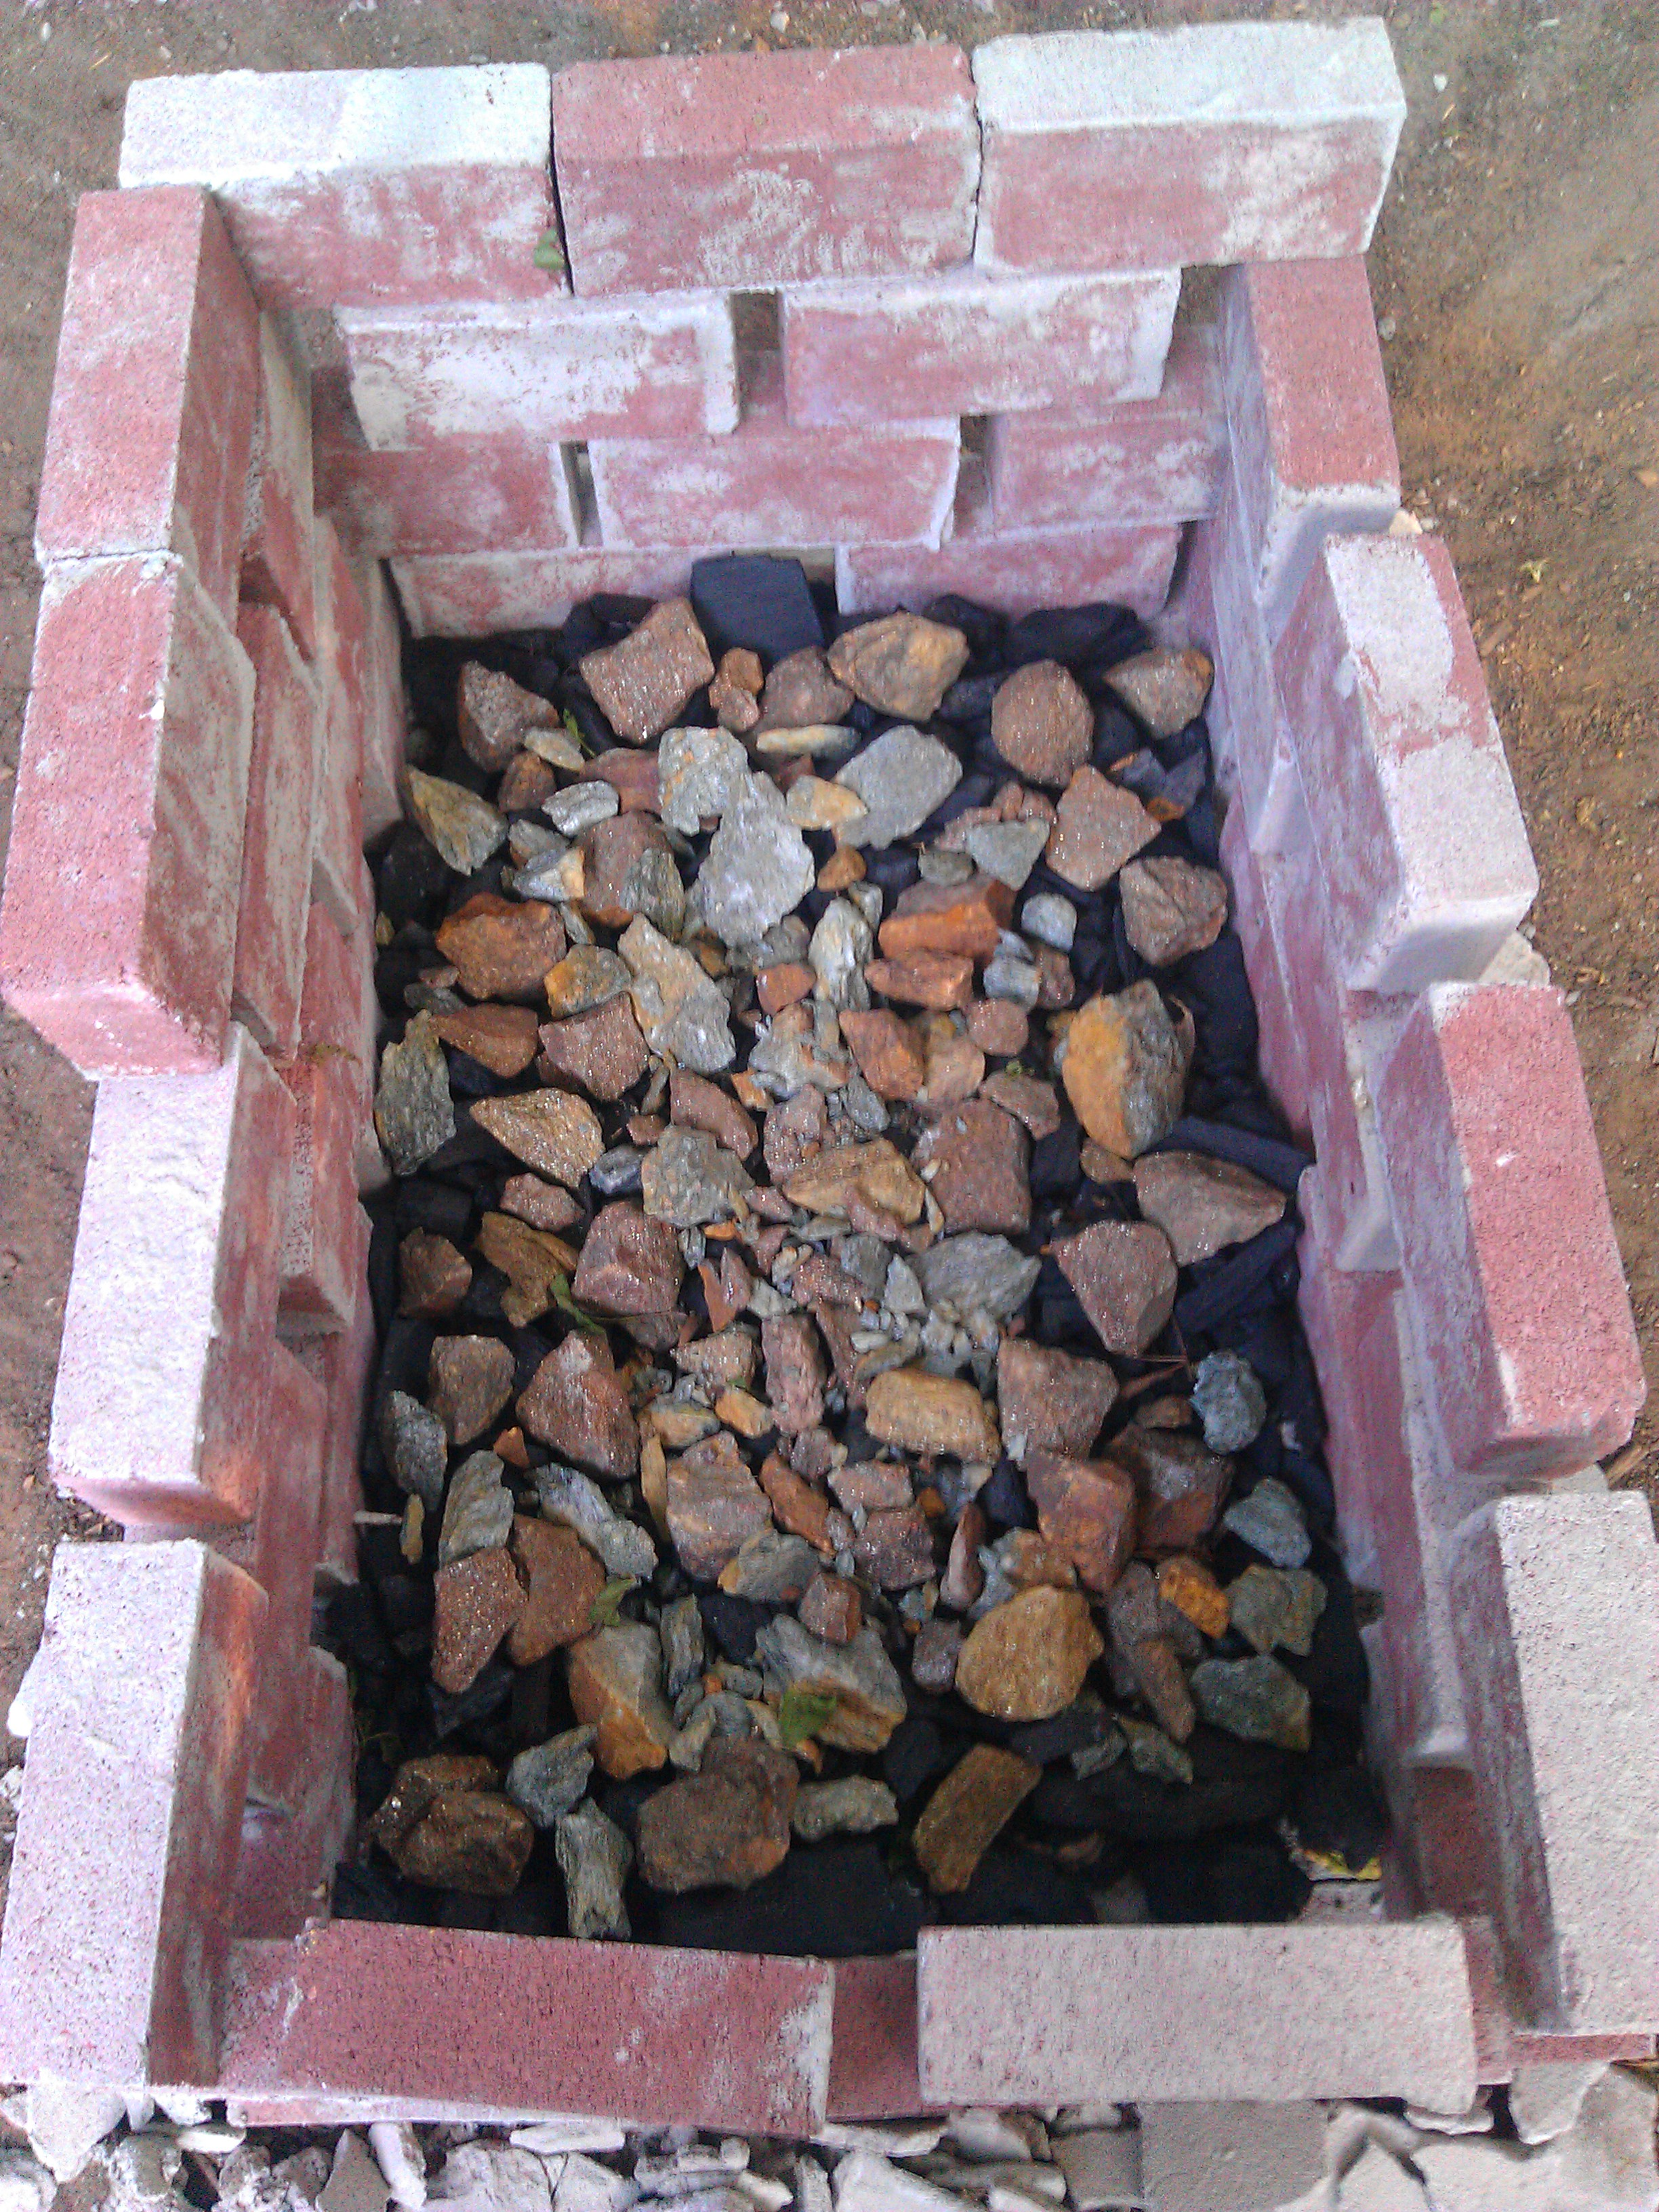
\includegraphics[width=3in]{images/2012.06.28_first_heap_roast/IMG_20120628_193016.jpg}
\label{fig:heaproast-a}
}
\subfigure[Second configuration.  Note open rear to direct airflow.]{
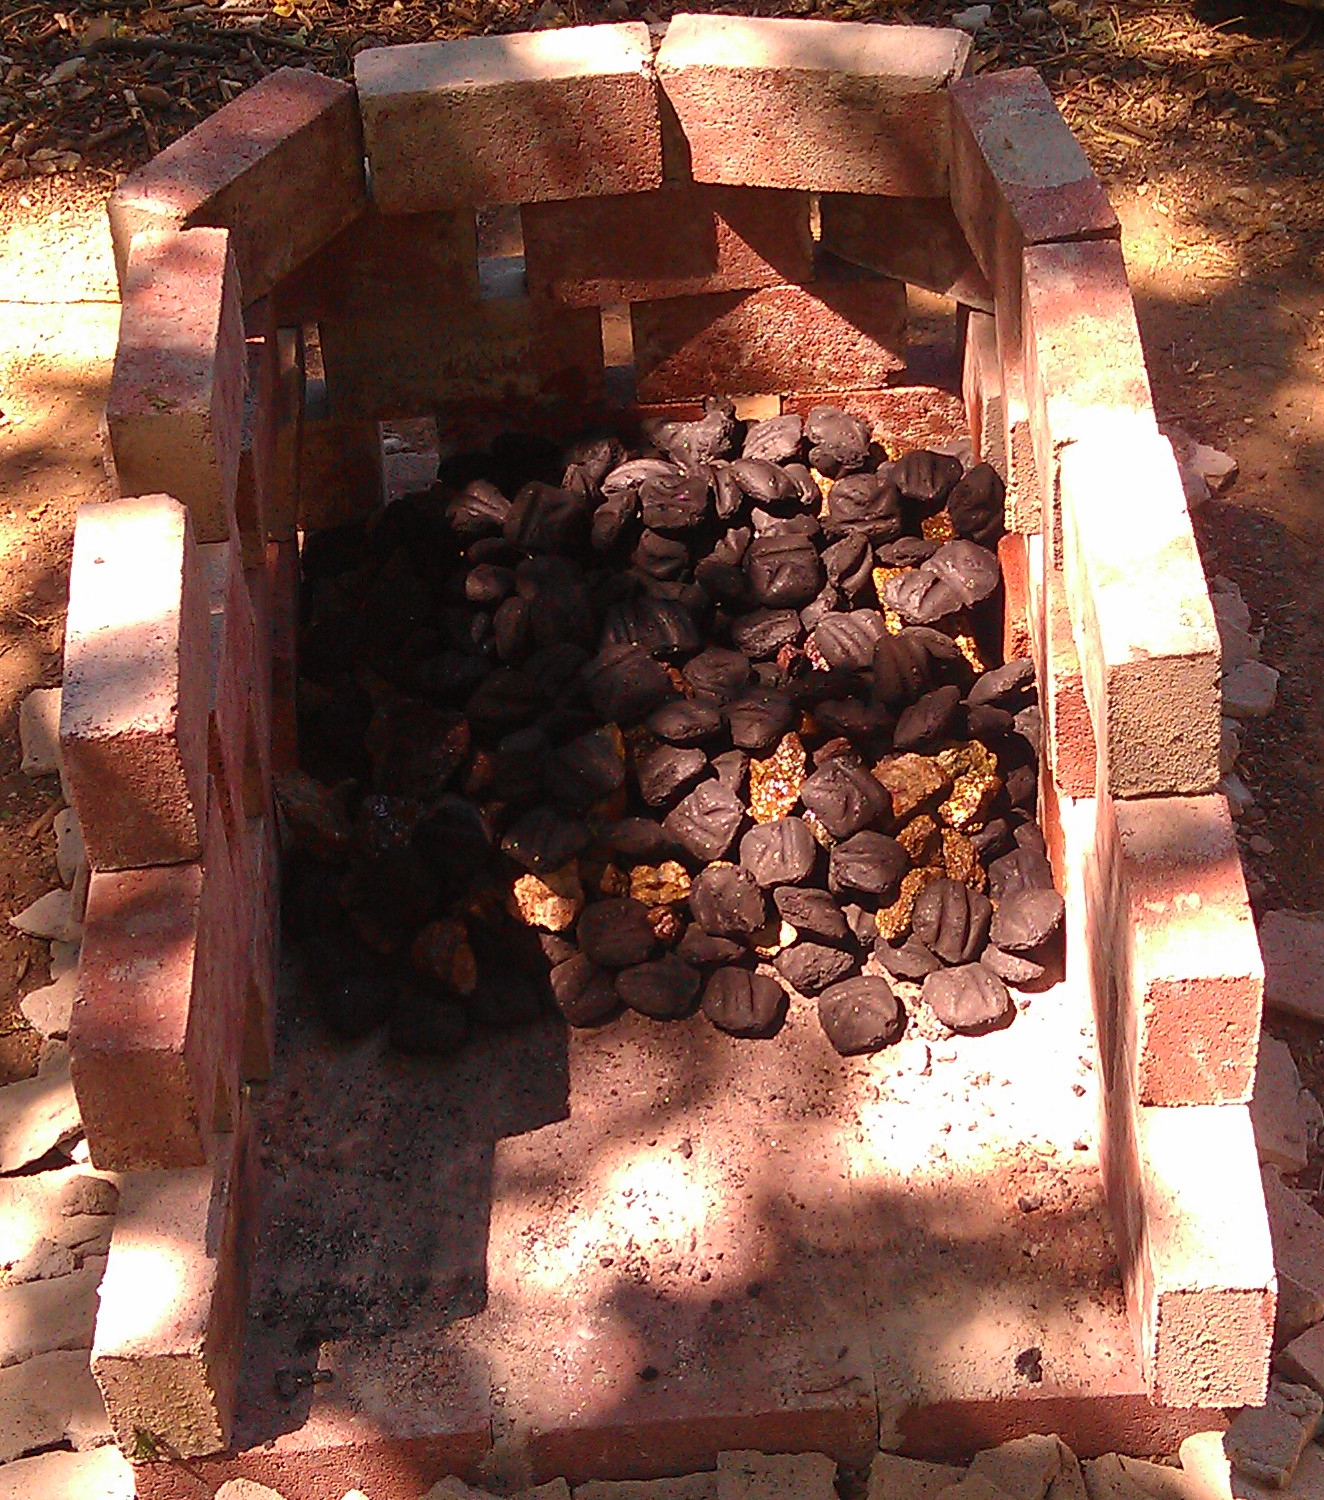
\includegraphics[width=3in]{images/2012.06.29_second_heap_roast/second_heap_roast.jpg}
\label{fig:heaproast-b}
}
\subfigure[Third configuration, using smaller fans and one airflow port.]{
\includegraphics[width=3in]{images/2012.06.30_third_heap_roast/third_roast_setup.jpg}
\label{fig:heaproast-c}
}
\subfigure[Fourth configuration, with four airflow channels.]{
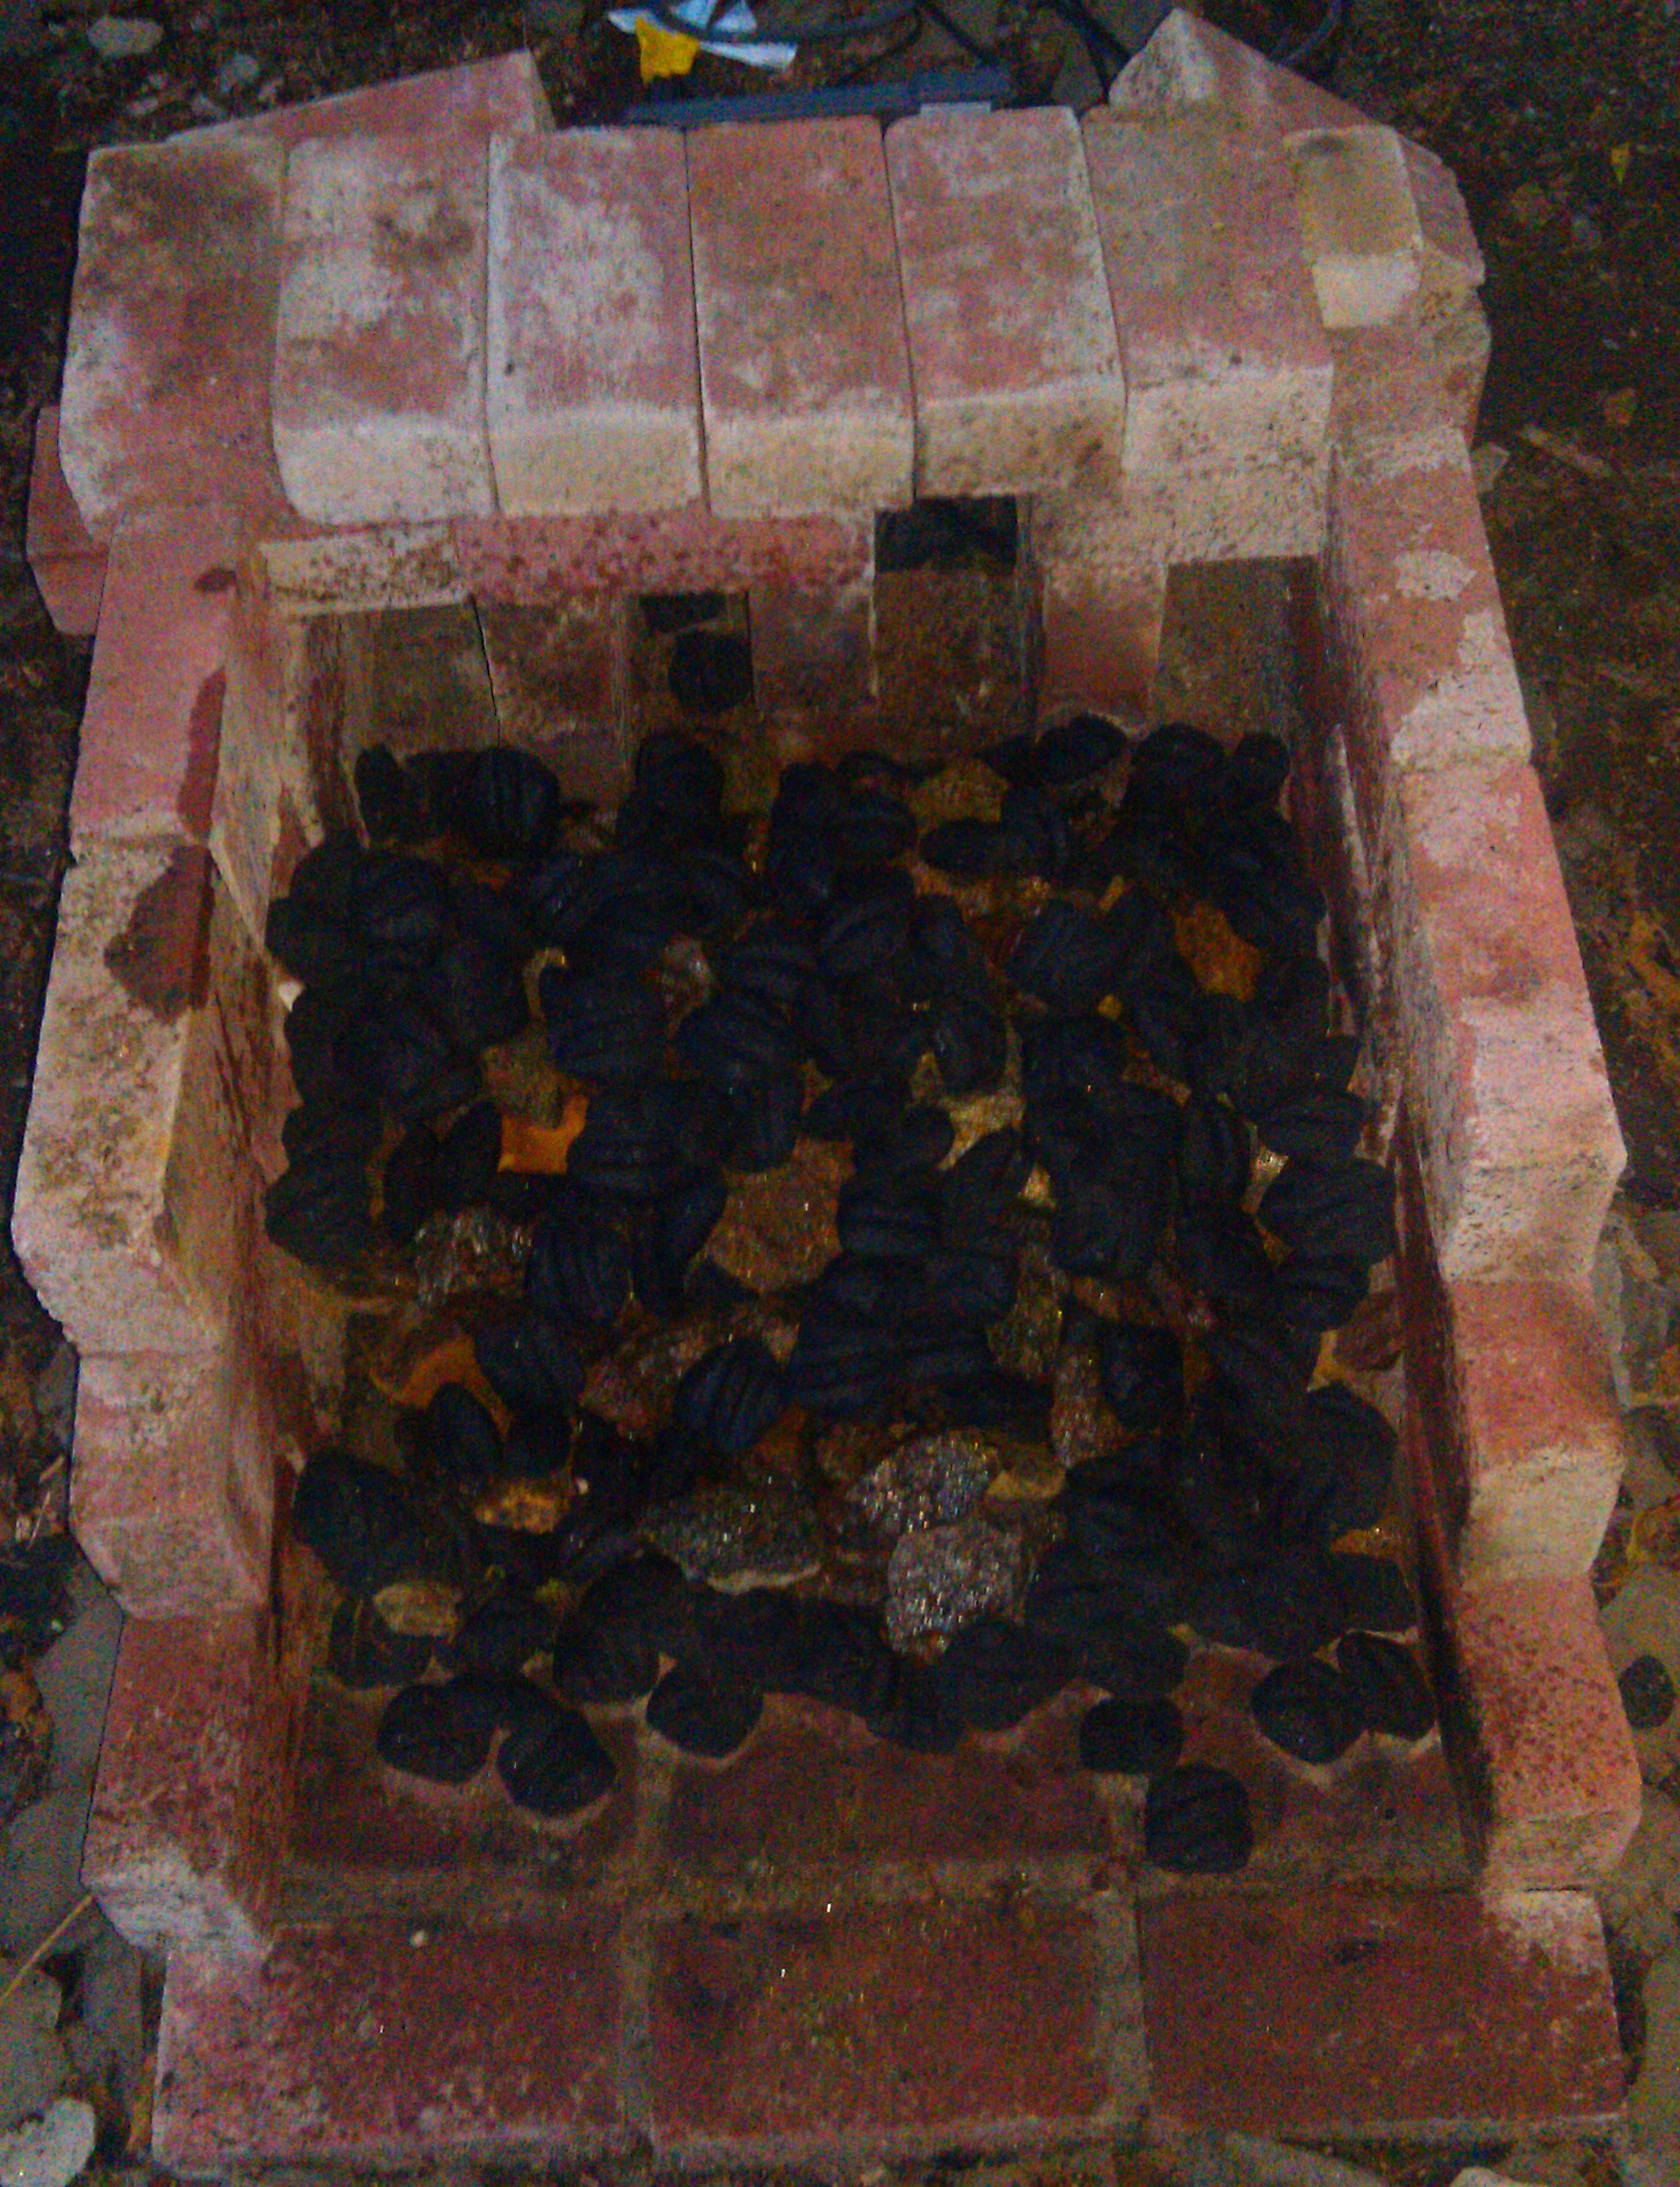
\includegraphics[width=3in]{images/2012.07.05_fourth_heap_roast/fourth_roast_setup.jpg}
\label{fig:heaproast-d}
}

\caption{Four heap roast configurations, given in chronological order of use.}
\label{fig:heaproast}
\end{figure}

\subsubsection{Initial Proof-Of-Concept}

As a first venture into roasting, a few small rocks (up to 1.5 inches in
diameter) were piled into a paint roller tray along with a handful of charcoal
and lit with the assistance of charcoal lighter fluid.  No forced airflow was
present, other than that provided by the lungs of the experimenters.  In this
setting the blue flame of the calcination process was not observed; however, the
sudden increase in heat caused by the onset of calcination was clear, and the
resultant ignition of the nearby ground forced the cancellation of the
experiment.  Due to the particularly short length of this trial (approximately
five minutes) it is unlikely that any significant quantity of ore was roasted.

Then, one ore fragment was taken and held over the open flame of a small camping
stove for approximately fifteen to twenty minutes.  While the rock did not
appear to be emitting flames of its own, the blue flames of the stove may have
simply made the flames of the rock impossible to see.  During this time, the
rock emitted sulfur dioxide (noticed by its pungent smell) and began to glow
red.  The temperature of the stove's flames is estimated at approximately
500$^\circ$C, giving the conclusion that the ore will glow at approximately the
temperature it roasts at.

After this trial, the rock was cracked open with very little force; far less
than would have been necessary for breakage before the roasting.  The rock had
changed from a grayish-red to a reddish-black with hints of a purple-like color
and a presence of small, white flecks.  This change was very obvious; however,
it is not known if this indicates the complete roasting of the ore.

\subsubsection{First Heap Roast}

This type of small-scale trial is simply insufficient for roasting any large
quantity of ore.  Therefore, a brick enclosure was designed.  This initial
enclosure can be seen in Figure \ref{fig:heaproast-a}.  The sidewalls were
intentionally left unmortared, so a fan could provide airflow through the holes
in the bricks.  For this setup, the mixture of charcoal fuel to ore chunks (by
volume) was approximately 1:1, with charcoal layered on the bottom and ore piled
on top.  The roast was started with the assistance of lighter fluid.

The release of sulfur dioxide began quickly -- within five minutes of the start
of the roast.  However, the characteristic blue flame of the calcining process
was not observed.  Generally, the charcoal fuel burned a orange-yellow color.
Unfortunately, the sulfur in the ore did not become the fuel source for the
roast, and the charcoal fuel was exhausted in approximately two and a half
hours.  Several different fan configurations were tried, including placing the
large fan directly on top of the brick walls, blowing downwards.  While very
effective at providing airflow for the hotter burning of the charcoal fuel, this
resulted in the melting of the plastic fan housing.

After the charcoal fuel was exhausted, the ore was allowed to cool and then was
inspected.  Most of the ore had visibly changed in the same manner as the
individually-roasted fragment from the previous section: a reddish-black
exterior (almost certainly \ce{FeO}) with a black interior with hints of purple
and small white flecks.  The reflective bits of metal were still present.

However, not all rocks exhibited these changes; only approximately half the
rocks had changed noticeably.  Those which did not change were later re-roasted.
These results have some similarity to those given by Peters \cite{peters1887},
but not much; this is most likely a result of the smaller roast size (20 to 30
pounds of ore, as opposed to hundreds of tons in Peters' documentation).  This
relative lack of ore likely results in lower heat than necessary to produce a
self-sustaining reaction of calcination.  Nonetheless, at least mildly positive
results were achieved.

\subsubsection{Second Heap Roast}

One of the main problems with the first trial was the direction of the sulfur
dioxide fumes.  Without particularly strong airflow, changing wind currents
would send the noxious gases in different directions, leaving nowhere to safely
stand to avoid the potentially arsenic-laced gas cloud.  Therefore, the main
modification to the design was to open the rear of the structure and push air in
that direction.  In addition, the charcoal to ore ratio was increased to
approximately 1.5:1, and fuel was piled both above and below the ore (in a
`sandwich'-like configuration).

These improvements were helpful; however, the airflow was not sufficient to
completely overpower even mild wind currents.  In general, the roast appeared to
be burning at a higher temperature (as observed by the colors emitted by the
charcoal fuel) and hints of blue flames were observed, although an actual
self-sustaining burning ore fragment was not seen.


\section{Smelting (Production of Blister Copper)}

% stuff


% There will probably be other sections.  But we're not there yet...

\section{Conclusion}

% Then the bibliography.

\end{document}
